\subsection*{Punto 01}

\textbf{Muestra en una gráfica el mínimo de la función objetivo como una función de k, para $k \in \{2, 3, 4, 5, 6\}$}

En la figura \ref{fig:problema_05_minimum_score} se visualiza la función objetivo obtenida para el dataset \file{creditcar.csv}. En esta se presenta una disminución en su valor conforme el número de clusters aumenta.

\begin{figure}[H]
    \centering
    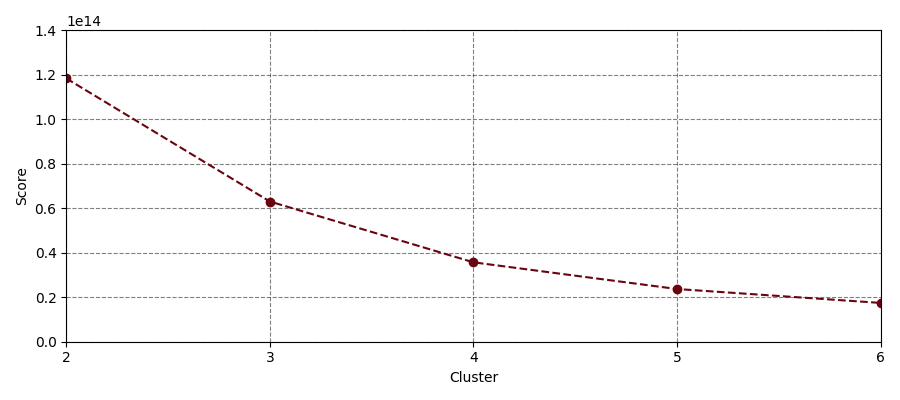
\includegraphics[width=16cm]{Graphics/Problema_05/minumum_score.png}
    \caption{Mínimo de la función objetivo para cada k calculada.}
    \label{fig:problema_05_minimum_score}
\end{figure}